\documentclass{jsarticle}
  \title{通常最小二乗法(Ordinary Least Squares: OLS)}
  \author{T.Chiba}
  \usepackage{latexsym}
  \usepackage[dvipdfmx]{graphicx}
  \usepackage{array, booktabs}
  \usepackage{float}
  \usepackage{moreverb}
  \usepackage{here}   %図の挿入場所を「ここ」で固定 H
  \usepackage{fancyvrb}
  %\usepackage{amsmath, amssymb,theorem}
  \usepackage{ascmac}
  \usepackage{geometry}%余白とか縮小するやつ
  \usepackage{bm}      %ベクトル
  \usepackage{cancel}  %文字の打ち消し線
  \usepackage{url}     %URL
  \usepackage{mathrsfs}%花文字 mathscr{ABCD...}
  \usepackage{comment} %複数行にわたるコメントアウトの実現 \begin{comment}~\end{commnet}
  \usepackage{mathtools}
  \usepackage{newtxtext,newtxmath, theorem} % フォント
  
  \geometry{left=30mm,right=30mm,top=25mm,bottom=25mm}
  
  \theoremstyle{plain}
   \newtheorem{theo}{定理}[section]
   \renewcommand{\thetheo}{}
   \newtheorem{defi}{定義}[section]
   \renewcommand{\thedefi}{}
   \newtheorem{lemm}{補題}[section]
   \renewcommand{\thelemm}{}
   \newtheorem{Proof}{証明}[section]
   \renewcommand{\theProof}{}
   \newtheorem{exam}{例}[section]
   \renewcommand{\theexam}{}
  \def\qed{\hfill $\Box$} %証明終わりの記号
  
  % 式番号に節番号を付加 (section.subsection)
  %\def\theequation{\thesection.\arabic{equation}}
  %\makeatletter
  %\@addtoreset{equation}{subsection}
  %\makeatother
  
  % section.subsection.subsection
  %\makeatletter
  % \renewcommand{\theequation}{%
  %   \thesubsection.\arabic{equation}}
  %  \@addtoreset{equation}{subsection}
  %\makeatother

  \begin{document}
  % タイトルの表示
  \maketitle
  \begin{abstract}
    最小二乗法についてみていく.
  \end{abstract}
  \section{最小二乗法(1変量)}
    本題に入る前に,リハビリもかねて1変量の最小二乗法を確認する.
    線形回帰モデルは下記のような構造をしていると考えられる.
  \begin{equation}
    y = \alpha + \beta x + \varepsilon
  \end{equation}
    $x, y$ についての観測値 $\{(x_i, y_i) | i = 1,2,\ldots,n\}$ がそれぞれ次のような構造を持っていると仮定する.
  \begin{equation}
    y_i = \alpha + \beta x_i + \varepsilon_i, i = 1,\ldots,n
  \end{equation}
  誤差 $\varepsilon$ の平方和を考える.
  \begin{equation}
    Q(\alpha, \beta) = \sum_{i=1}^n \varepsilon_i^2 = \sum_{i=1}^n \{y_i - (\alpha + \beta x_i) \}^2
  \end{equation}
  これを.偏差平方和と呼ぶ.$Q(\alpha, \beta)$ を最小にするような $\alpha = \hat{\alpha}, \beta = \hat{\beta}$ を最小二乗推定量(Least Squares Estimator: LSE)と呼ぶ.

  \begin{equation}
  \label{Normal-equation-2-value}
    \begin{cases}
      \frac{\partial Q(\alpha, \beta)}{\partial \alpha} = 0 \\
      \frac{\partial Q(\alpha, \beta)}{\partial \beta} = 0
    \end{cases}
  \end{equation}
  を満たすような $\alpha, \beta$ を考える. 2階の偏微分まで計算すると,
  \begin{eqnarray}
    \frac{\partial Q}{\partial \alpha} &=& -2 \sum_{i=1}^n (y_i - \alpha - \beta x_i) \\
    \frac{\partial^2 Q}{\partial \alpha^2} &=& 2n > 0 \\
    \frac{\partial Q}{\partial \beta} &=& -2\sum_{i=1}^n x_i (y_i - \alpha - \beta x_i) \\
    \frac{\partial^2 Q}{\partial \beta^2} &=& 2 \sum_{i=1}^n x_i^2 >= 0 \\
    \frac{\partial^2 Q}{\partial \alpha \partial \beta} &=& 0
  \end{eqnarray}
  ヘッセ行列は,
  \begin{equation}
    H = 
    \left[
      \begin{array}{cc}
        \partial^2 Q / \partial \alpha^2 & \partial^2 Q/\partial \alpha \partial \beta \\
        \partial^2 Q/\partial \alpha \partial \beta & \partial^2 Q / \partial \beta^2
      \end{array}
    \right]
    = \left[
      \begin{array}{cc}
        2n & 0 \\
        0 & 2 \sum x_i^2
      \end{array}
    \right]
  \end{equation}
  いま, 任意の2次元ベクトル $\bm{t} = (t_1, t_2)'$ に対して二次形式,
  \begin{equation}
    \bm{t}'H\bm{t} = (t_1, t_2) \left(
      \begin{array}{cc}
        2n & 0 \\
        0 & 2 \sum x_i^2
      \end{array}
    \right) \left( 
      \begin{array}{c}
        t_1 \\
        t_2
      \end{array}
    \right) = 2\left(nt_1^2 + t_2^2 \sum x_i^2 \right) \geq 0
  \end{equation}
  となり, これが $0$ となるのは, $\bm{t}=\bm{0}$ のときのみ. よってヘッセ行列 $H$ は正定値. つまり, 式(\ref{Normal-equation-2-value}) を満たす,
  $\alpha, \beta$ が極小値であることが分かる. また, 図 \ref{fig:Quadratic-function-of-bivariate-function} の形から, 極小かつ最小であることも分かる.

  \begin{figure}[htbp]
    \centering
    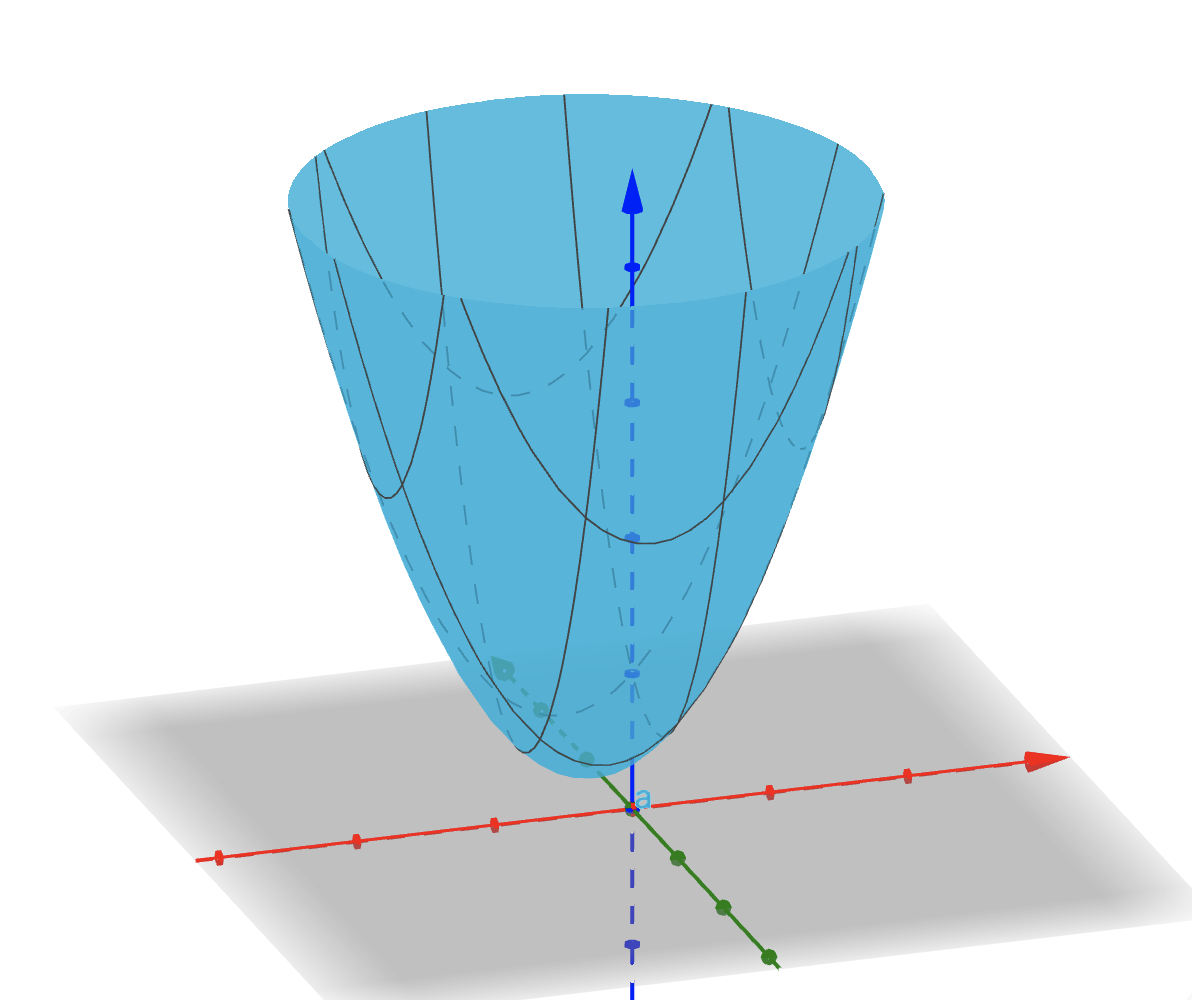
\includegraphics[scale=0.5]{img/Quadratic-function-of-bivariate-function.png}
    \caption{2変数関数の二次関数のイメージ}
    \label{fig:Quadratic-function-of-bivariate-function}
  \end{figure}

  式(\ref{Normal-equation-2-value}) を解いていく.

  \begin{eqnarray}
    &&
    \begin{cases}
      \frac{\partial Q}{\partial \alpha} = -2 \sum (y_i - \alpha - \beta x_i) = -2 \left\{ \sum y_i - n\alpha - \beta \sum x_i \right\} = 0 \\
      \frac{\partial Q}{\partial \beta} = -2\sum_{i=1}^n x_i (y_i - \alpha - \beta x_i) = -2 \left\{ \sum x_i y_i  - \alpha \sum x_i - \beta \sum x_i^2 \right\} = 0
    \end{cases} \\
    &\Leftrightarrow&
    \begin{cases}
      \alpha n + \beta \sum x_i = \sum y_i \\
      \alpha \sum x_i + \beta \sum x_i^2 = \sum x_i y_i
    \end{cases}
  \end{eqnarray}

  よって,

  \begin{equation}
    \hat{\alpha} = \frac{1}{n} \sum y_i - \hat{\beta} \frac{1}{n} \sum x_i = \bar{y} - \hat{\beta}
  \end{equation}

  \begin{eqnarray*}
    \hat{\alpha} \sum x_i + \beta \sum x_i^2 &=& \sum x_i y_i
    (\bar{y} - \beta \bar{x}) \bar{x} \sum x_i^2 &=& \frac{1}{n} x_i y_i
    \bar{y} \bar{x} - \beta 
  \end{eqnarray*}


  \appendix
  \section{}
  \subsection{2変数関数の極値}
  偏差平方和を最小にするような, $\alpha$ と $\beta$ を求める際に,$\alpha, \beta$ に関する偏微分を $0$ として,推定量を求めた.しかし,偏微分が $0$ と置くだけでは,
  $Q(\alpha, \beta)$ の極値が求められるだけで,最小値かどうかは分からない.テキストだと当たり前のように書かれているけど.

  \subsubsection{極大・極小}
  関数 $f(x, y)$ は連続かつ微分可能とする.
  \begin{lemm}
  境界点\footnotemark でない極大点, 極小点においては
    \begin{equation}
      \frac{\partial f}{\partial x}(x_0, y_0) = 0, \frac{\partial f}{\partial y}(x_0, y_0) = 0
    \end{equation}
  となる.
  \footnotetext{~\cite{bibun-sekibun} p18 参照.}
  \end{lemm}
  \begin{Proof}
  もし $\frac{\partial f}{\partial x}(x_0, y_0) \neq 0$ ならば、微分可能性の定義\footnotemark
    \begin{equation*}
      \begin{cases}
        f(x, y) - f(x_0, y_0) = \frac{\partial f}{\partial x}(x_0, y_0)(x - x_0) + \frac{\partial f}{\partial y}(x_0, y_0)(y - y_0) + g(x, y), \\
        \lim_{\bm{x} \to \bm{x}_0} \frac{g(x, y)}{|\bm{x} - \bm{x}_0 |} = 0
      \end{cases}
    \end{equation*}
    において, $y = y_0$ と置くと,
    \begin{eqnarray*}
      f(x, y_0) - f(x_0, y_0) &=& \frac{\partial f}{\partial x}(x_0, y_0)(x - x_0) + g(x, y_0) \\
       &=& \frac{\partial f}{\partial x}(x_0, y_0)(x - x_0)\left\{ 1 + c \cdot \frac{g(x, y_0)}{x - x_0} \right\}
    \end{eqnarray*}
    右辺の $\{  \}$ の中は $x$ が $x_0$ に十分近いとき $> 0$ となる. 一方, $x - x_0$ は $x$ が $x_0$ の近傍を動く時必ず符号を変えるため, 
    $f(x_0, y_0)$ は極大値でも極小値でもないことが分かる. $\frac{\partial f}{\partial y}(x_0, y_0) \neq 0$ としても同様.

    これにより, 連立方程式
    \begin{equation*}
      \frac{\partial f}{\partial x}(x_0, y_0) = 0, \frac{\partial f}{\partial y}(x_0, y_0) = 0
    \end{equation*}
    を解けば, 境界点でない極値の候補者が全て見つかる. \qed
  \end{Proof}
  \footnotetext{
    $z = f(x, y)$ が点 $\bm{x}_0 = (x_0, y_0)$ で微分可能であるとは, ある定数 $\alpha, \beta$ があって,
    \begin{equation*}
      \begin{cases}
        f(x, y) = f(x_0, y_0) + \alpha(x - x_0) + \beta(y - y_0) + g(x, y) & \\
        \lim_{\bm{x} \to \bm{x_0}} \frac{g(x, y)}{| \bm{x} - \bm{x}_0 |} & (\bm{x} = (x, y) \neq \bm{x}_0)
      \end{cases}
    \end{equation*}
    と表せること(~\cite{bibun-sekibun} p153 参照)
  }

  \subsubsection{極大・極小の判定}
  極大値か極小値かの判定はヘッセ行列により行うことができる.

  \begin{defi}[ヘッセ行列]
    行列
    \begin{equation*}
      \left[
        \begin{array}{cc}
          f_{xx} & f_{xy} \\
          f_{xy} & f_{yy}
        \end{array}
      \right]
    \end{equation*}
    を $f(x, y)$ に関するヘッセ行列という.
  \end{defi}

  \begin{theo}
    $\frac{\partial f}{\partial x}(x_0, y_0) = \frac{\partial f}{\partial 0}(x_0, y_0) = 0$ を満たす点 $x_0, y_0$ においてヘッセ行列が\footnotemark
    \begin{description}
      \item[正定値] $(x_0, y_0)$ は極小値
      \item[負定値] $(x_0, y_0)$ は極大値
      \item[不定値] $(x_0, y_0)$ は極値点ではない
    \end{description}
  \end{theo}
  \footnotetext{高校数学の美しい物語とか参考になる:\url{https://mathtrain.jp/hessian}}

  \subsubsection{正定値・負定値・不定値}
  $\bm{x}'\bm{A}\bm{x}$ を任意の二次形式とする. ただし, $\bm{x} = (x_1, \ldots, x_n)'$.
  
  \begin{description}
    \item[非負定値(nonnegative definite)] $\mathcal{R}^n$\footnotemark のあらゆる $\bm{x}$ に対して $\bm{x}'\bm{A}\bm{x} \geq 0$ であるとき. $\bm{x}$ の少なくとも1つの値, 具体的には $\bm{x} = \bm{0}$ に対して, $\bm{x}'\bm{A}\bm{x} = 0$ であることに注意.
    \item[正定値(positive definite)] $\bm{x}'\bm{A}\bm{x}$ が非負定値かつ, 零ベクトル $\bm{0}$ に対してのみ $\bm{x}'\bm{A}\bm{x} = 0$ となる時. すなわち, $\bm{x} = \bm{0}$ を除く, あらゆる $\bm{x}$ に対して $\bm{x}'\bm{A}\bm{x} > 0$ のとき.
    \item[半正定値(positive semidefinite)] 非負定値であるが, 正定値でない二次形式. あらゆる $\bm{x} \in \mathcal{R}^n$ に対して, $\bm{x}'\bm{A}\bm{x} \geq 0$で, ある $\bm{x} \neq \bm{0}$ に対して $\bm{x}'\bm{A}\bm{x} = 0$ のとき.
    \item[非正定値, 負定値, 半負定値]  それぞれ, $-\bm{x}'\bm{A}\bm{x}$ が, 非負定値, 正定値, 半正定値のとき.
    \item[不定値(indefinite)] 非負定値でも, 非正定値でもない二次形式.
  \end{description}
  \footnotetext{
    記号 $\mathcal{R}^{m \times n}$ はその要素が全ての $m \times n$ 行列からなる線形空間を表す. 記号 $\mathcal{R}^n$ は全ての $n$ 列次元ベクトルの集合.
  }

  \begin{thebibliography}{9}
    \bibitem{finance-stats} Tze Leung Lai, Haipeng Xing 著, 松原 望, 山村吉信 訳: 『ファイナンスのための統計学 -統計的アプローチによる評価と意思決定-』, 東京図書, 2016
    \bibitem{math-data-analysis} 鈴木 武, 山田 作太郎:『数理統計学 -基礎から学ぶデータ解析』, 内田老鶴圃, 1996
    \bibitem{Inagaki} 稲垣宣生:『数学シリーズ 数理統計学(改訂版)』, 裳華房, 2003
    \bibitem{daigaku-biseki} 江川博康:『弱点克服 大学生の微積分』東京図書, 2005
    \bibitem{bibun-sekibun} 笠原晧司: 『サイエンスライブラリー 数学=12 微分積分学』, サイエンス社, 1974
    \bibitem{Matrix-Algebra} David A. Harville, (監訳)伊里正夫 : 『統計のための行列代数(上)』,丸善出版, 2016
  \end{thebibliography}
\end{document}
